\documentclass[a4paper,10pt,twocolumn,uplatex]{jsarticle}
\usepackage{style/campus_presen_resume}
\usepackage{multirow}
\usepackage{hhline}
\usepackage{comment} 
\usepackage{scalefnt}
\usepackage{cite}

% \newenvironment{minilinespace}{
% \baselineskip = 4mm
% }

%---------------------------------------------------------------------
%レジュメ種別・日付設定(要変更)
%type 1:修士論文諮問会 2:卒業論文発表会 else:月例発表会
\type{3}
\year{2021}
\month{4}
\date{1}

%---------------------------------------------------------------------
%ページ番号設定(要変更)
\setcounter{page}{11}

%---------------------------------------------------------------------
\begin{document}

%---------------------------------------------------------------------
%タイトル作成部分(要変更)
%\maketitle{タイトル}{title}{名前}{name}{NAME}
\maketitle{タイトルタイトルタイトル}
{Title Title Title}
{山田 太郎}
{Taro Yamada}

%---------------------------------------------------------------------
\section{はじめに}
車載センサから得られたデータはダイナミックマップを管理するサーバに送信され,それに基づいて協調型自動運転を実現するアプリケーションが動作する.そのため,車両から送信される動的情報は常にサーバへと送信される必要があり,サーバは低遅延でデータを処理し,車両に送信する必要がある.また,一般に車両は100ミリ秒周期でダイナミックマップに送信する\cite{ITSinterval}.しかし,ダイナミックマップが扱う車両台数は膨大で,すべての車両が高頻度にデータを送信し続けると輻輳が懸念される.また,一般車車両と緊急車両から送信されるデータを同等に扱うと,交通安全サービスに支障をきたす恐れがある.\par
そこで,優先処理機能を用いることで車両の送信するデータを効率的に通信・処理することが期待できる.優先処理機能として,車両側で送信間隔を調整する方法と,データを受信・処理するサーバ側でデータの処理を調整する方法がある.通信の輻輳を考えると,車両側で送信間隔を調整することで効率化が期待できるが,我々はエッジを用いたダイナミックマップを検討しており,サーバでの処理がボトルネックとなる.そこで,車両から大量に送信されるデータに対して優先度を決定し,各優先度に応じたQoSによる優先処理機能を実現し,有効性を検討する.

%---------------------------------------------------------------------
\section{エッジを配置したダイナミックマップ}
エッジの配置にはいくつかの議論があるが,携帯電話基地局周辺に設置するモデルが有力であり,本研究ではそのモデルに従い,移動する車両からデータを送受信する携帯電話基地局に該当する位置にエッジを配置する.本ダイナミックマップは,クラウド,エッジ,車両の三層構造からなりこれらをノードと呼ぶ.クラウドでは広域的情報,エッジではリアルタイムな処理が必要な局所的情報を管理する.\par
欧州で標準化が進む協調型ITSシステムと同様に,各ノードは固有のIDを持ち,それぞれの通信部を通じて通信を行い,送受信されたデータは各ノードのアプリケーションで処理・実行される.ダイナミックマップでは大量のデータをリアルタイムに送受信する必要があるため,各ノードはUDPを用いて通信を行う.また,各エッジはマルチキャストを利用することで,送信先となる車両のIPアドレスの設定なくデータを送信することができる.各車両は,車両からエッジにデータを送信する際の宛先IPアドレスとしてエニキャストアドレスを使用することで,車両はどこにいても,クラウドやエッジのネットワーク構成を意識することなく,最寄りのエッジにデータを直接送信することが可能となる.

%---------------------------------------------------------------------
\section{QoS優先制御}
\subsection{概要}
車両から高頻度で送信されるデータは最寄りのエッジで受信される.データを受信したエッジは,その車両を管轄するエッジが自身かを判断し,自身であれば車両の優先度に応じたキューにデータを格納する.この優先度は,救急車などの優先車両を高優先,路線バスなどを公共交通機関を中優先,自家用車を低優先としている.エッジは,各キューに格納されているデータを随時アプリケーションに送信し,アプリケーションを実行する必要がある.しかし,各エッジが管理する車両台数は膨大で,各車両が高頻度でデータを送信するため処理遅延が懸念される.エッジは,キューに格納されているデータのうち,高優先のデータは確実にアプリケーションにリアルタイムに送信する必要がある.そこで,QoSを用いて高優先のデータをアプリケーションに送信,またエッジに実装されている高優先アプリケーションを実行する.本研究で構築するQoS優先制御を用いたダイナミックマップの構成を図\ref{fig:qos-overview}に示す.

\begin{figure*}[!t]
\centering%
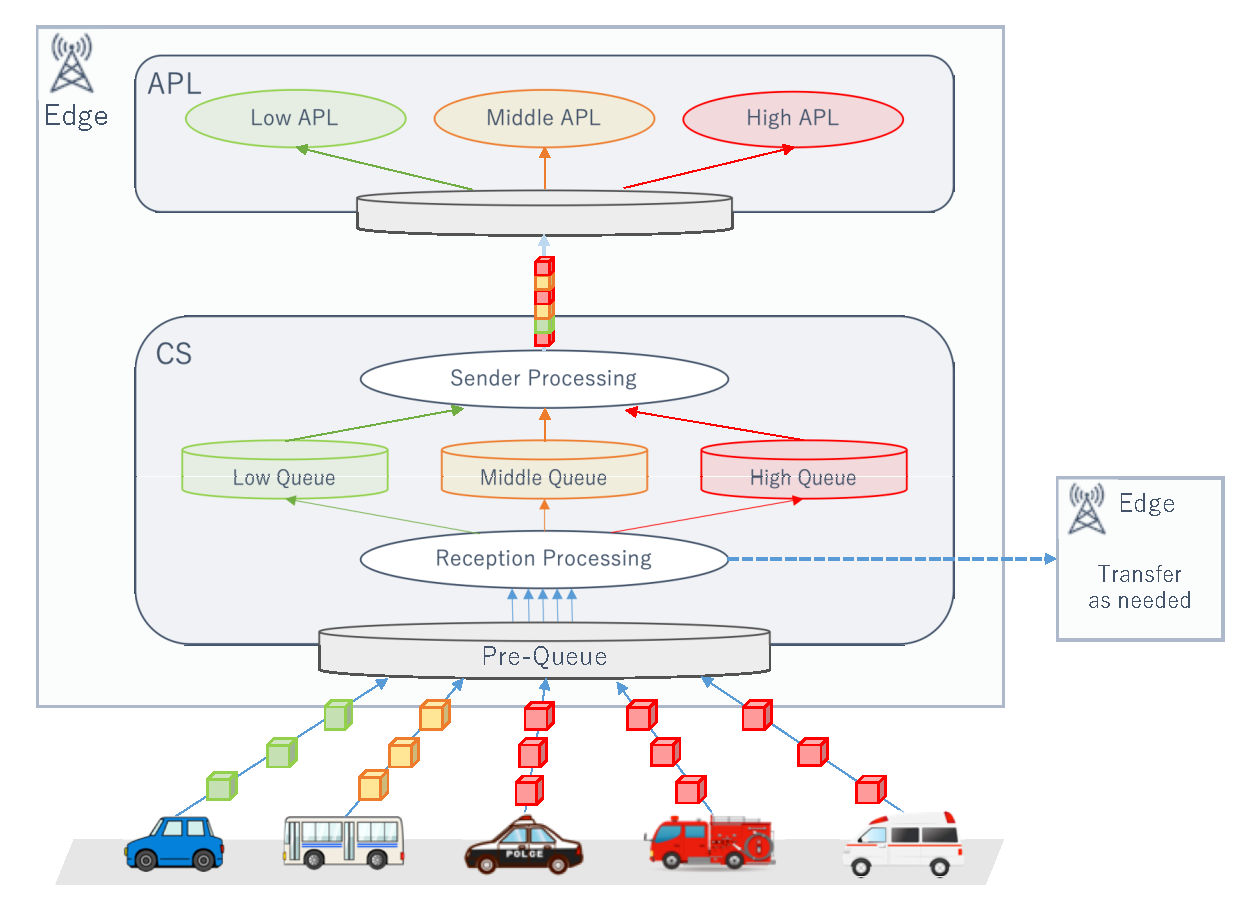
\includegraphics[width=0.7\linewidth]{img/QoSoverview.eps}
\caption{Overview of QoS Processing}
\label{fig:qos-overview}
\end{figure*}

%---------------------------------------------------------------------
\subsection{データの種類による優先制御}
\label{sec:data-priority}
エッジは,各優先度ごとのキューに格納されているデータを随時取り出し,アプリケーションに送信する必要がある.通常は,全ての車両データに対して最も古いデータから取り出すが,これでは緊急車両等の高優先のデータがリアルタイムに通信・処理できない可能性がある.そこで,Strict PriorityとWeighted Round Robinを用いてキューに格納されたデータを効率的に取り出す手法を検討する.\par
Strict Priorityを用いた場合,高優先キューのデータが増加すると低優先キューのデータが溜まりやすいという問題がある.しかし,日本において自家用車に対する緊急車両の台数は1\%以下であることから\cite{EmergencyCars},高優先キューのデータをリアルタイムに送信するためにStrict Priorityによる優先制御を検討する.

%---------------------------------------------------------------------
\subsection{輻輳時のパケット破棄}
\ref{sec:data-priority}章では,道路上を走行する車両の種類によって優先度を設定し,各車両から送信されたデータを受信したエッジが優先度に応じてキューからデータを取り出す手法を提案した.Strict Priorityを用いた優先制御によって,緊急車両等の高優先データは高信頼でリアルタイムに送信することが可能となる.しかし,電波状況や交通環境の影響によってエッジが管轄する車両台数が増加した場合に,処理遅延が発生する可能性がある.処理遅延が発生すると,エッジはデータをキューに格納し続けるため,データごとの遅延時間が増加し続ける.移動し続ける車両を管理するダイナミックマップにおいて,リアルタイム性は非常に重要であり,これは重大な問題となる.そこで,Tail DropやRandom Early Detectionを用いて輻輳時にパケットを破棄する機能を検討する.\par
ダイナミックマップにおいて,通信・処理のリアルタイム性は非常に重要であり,Tail Dropでは一度キューに格納したデータが確実に処理される信頼性はあるものの,データごとの遅延が大きくなる.そこで,Random Early Detectionを用いることで所々データが破棄される可能性はあるが,常に新たなデータをキューに格納することが可能となり,リアルタイム性の向上が期待できる.

%---------------------------------------------------------------------
\subsection{車両ごとの優先度決定}
QoS制御を実現するためには,各車両に対して優先度を決定する必要がある.今回は,2.1章で述べたように緊急車両を高優先,公共交通機関を中優先,自家用車を低優先とした.比較的予測不可能な行動をしやすい高齢者が運転する車などの存在を検討する必要はあるが,ダイナミックマップが基本的に自動運転車を対象としていること,本研究ではあくまでQoS優先制御による通信環境の効率化を検討していることから本質ではなく,言及しないこととする.

%---------------------------------------------------------------------
\section{評価}
QoS優先制御によるダイナミックマッププラットフォームの通信環境について有効性を評価する.ダイナミックマップにおいて効率化によって安全性が失われてはいけない.そのため,効率性と安全性の評価が必要である.そこで,ダイナミックマップの各プロセスにおける処理遅延時間と各キューサイズ値を計測することで効率性を評価する.また,車両から送信されるデータのアプリケーションへの到達率と処理遅延時間を計測することで安全性を評価する.

%---------------------------------------------------------------------
\section{まとめ}
本研究では,サーバ・車両からなるダイナミックマッププラットフォームを構築し,再送機能を構築することで高い信頼性のある通信を実現した.また,レーンID毎に優先度を設定し,送信間隔を調整する優先処理機能を構築・検討した.評価の結果,提案手法ではレーンIDによる管理や優先処理機能がない場合に比べてスループットが向上した.

%---------------------------------------------------------------------
{
\footnotesize
\begin{thebibliography}{99}

\bibitem{ITSinterval}
一般財団法人 日本自動車研究所, "ITS 協調システムの情報項目の標準化に関する分析・検証 報告書", 2014.

\bibitem{EmergencyCars}
一般財団法人 自動車検査登録情報協会,https://www.airia.or.jp/index.html.

\end{thebibliography}
}

%---------------------------------------------------------------------
\end{document}

%---------------------------------------------------------------------